%%%%%%%%%%%%%%%%%%%%%%%%%%%%%%%%%%%%%%%%%%%%%%%%%%%%%%%%%%%%%%%%%%%%%%%%%%%%%%%%
%
%  Project: Sumcheck Protocol 
%
%  Authors:  Azucena Garvia <zucegb@gmail.com>
%		   Christoph Sprenger <sprenger@inf.ethz.ch>
%		   Jonathan Bootle <jbt@zurich.ibm.com>
%  
%%%%%%%%%%%%%%%%%%%%%%%%%%%%%%%%%%%%%%%%%%%%%%%%%%%%%%%%%%%%%%%%%%%%%%%%%%%%%%%%

\documentclass[11pt,a4paper]{article}
\usepackage{isabelle,isabellesym}

% additional packages
\usepackage{graphicx}       % to display session graph
\usepackage{a4wide}
\usepackage{verbatim}
% have each section start on a fresh page
\renewcommand{\isamarkupsection}[1]{\newpage\section{#1}}

% this should be the last package used
\usepackage{pdfsetup}

% for special symbols 
\usepackage{amssymb}

% urls in roman style, theory text in math-similar italics
\urlstyle{rm}
\isabellestyle{it}


\begin{document}

\title{The Sumcheck Protocol}
\author{Azucena Garvia, Christoph Sprenger and Jonathan Bootle}

\maketitle

\begin{abstract}
The sumcheck protocol, first introduced in 1992, is an interactive proof which is a key component of many probabilistic proof systems in computational complexity theory and cryptography, some of which have been deployed. We provide a formally verified security analysis of the sumcheck protocol, following a general and modular approach.

First, we give a general formalization of public-coin interactive proofs. We then define a \emph{generalized sumcheck protocol} for which we axiomatize the underlying mathematical structure and we establish its soundness and completeness. Finally, we prove that these axioms hold for multivariate polynomials, the original setting of the sumcheck protocol.
%
Our modular analysis will facilitate formal verification of sumcheck instances based on different mathematical structures with little effort, by simply proving that these structures satisfy the axioms.
%
Moreover, the analysis will encourage the development and formal verification of future probabilistic proof systems using the sumcheck protocol as a building block.

The paper presenting this formalization is to appear at CSF 2024 under the title ``Formal Verification of the Sumcheck Protocol''.
\end{abstract}


\tableofcontents

\newpage


% sane default for proof documents
\parindent 0pt\parskip 0.5ex

% display the theory dependency graph
%%%%%%%%%%%%%%%%%%%%%%%%%%%%%%%%%%%%%%%%%%%%%%%%%%%%%%%%%%%%%%%%%%%%%%%%%%%%%%%%
%
%  Project: Sumcheck Protocol 
%
%  Authors:  Azucena Garvia <zucegb@gmail.com>
%		   Christoph Sprenger <sprenger@inf.ethz.ch>
%		   Jonathan Bootle <jbt@zurich.ibm.com>
%  
%%%%%%%%%%%%%%%%%%%%%%%%%%%%%%%%%%%%%%%%%%%%%%%%%%%%%%%%%%%%%%%%%%%%%%%%%%%%%%%%

\begin{figure}[p]
  \begin{center}
    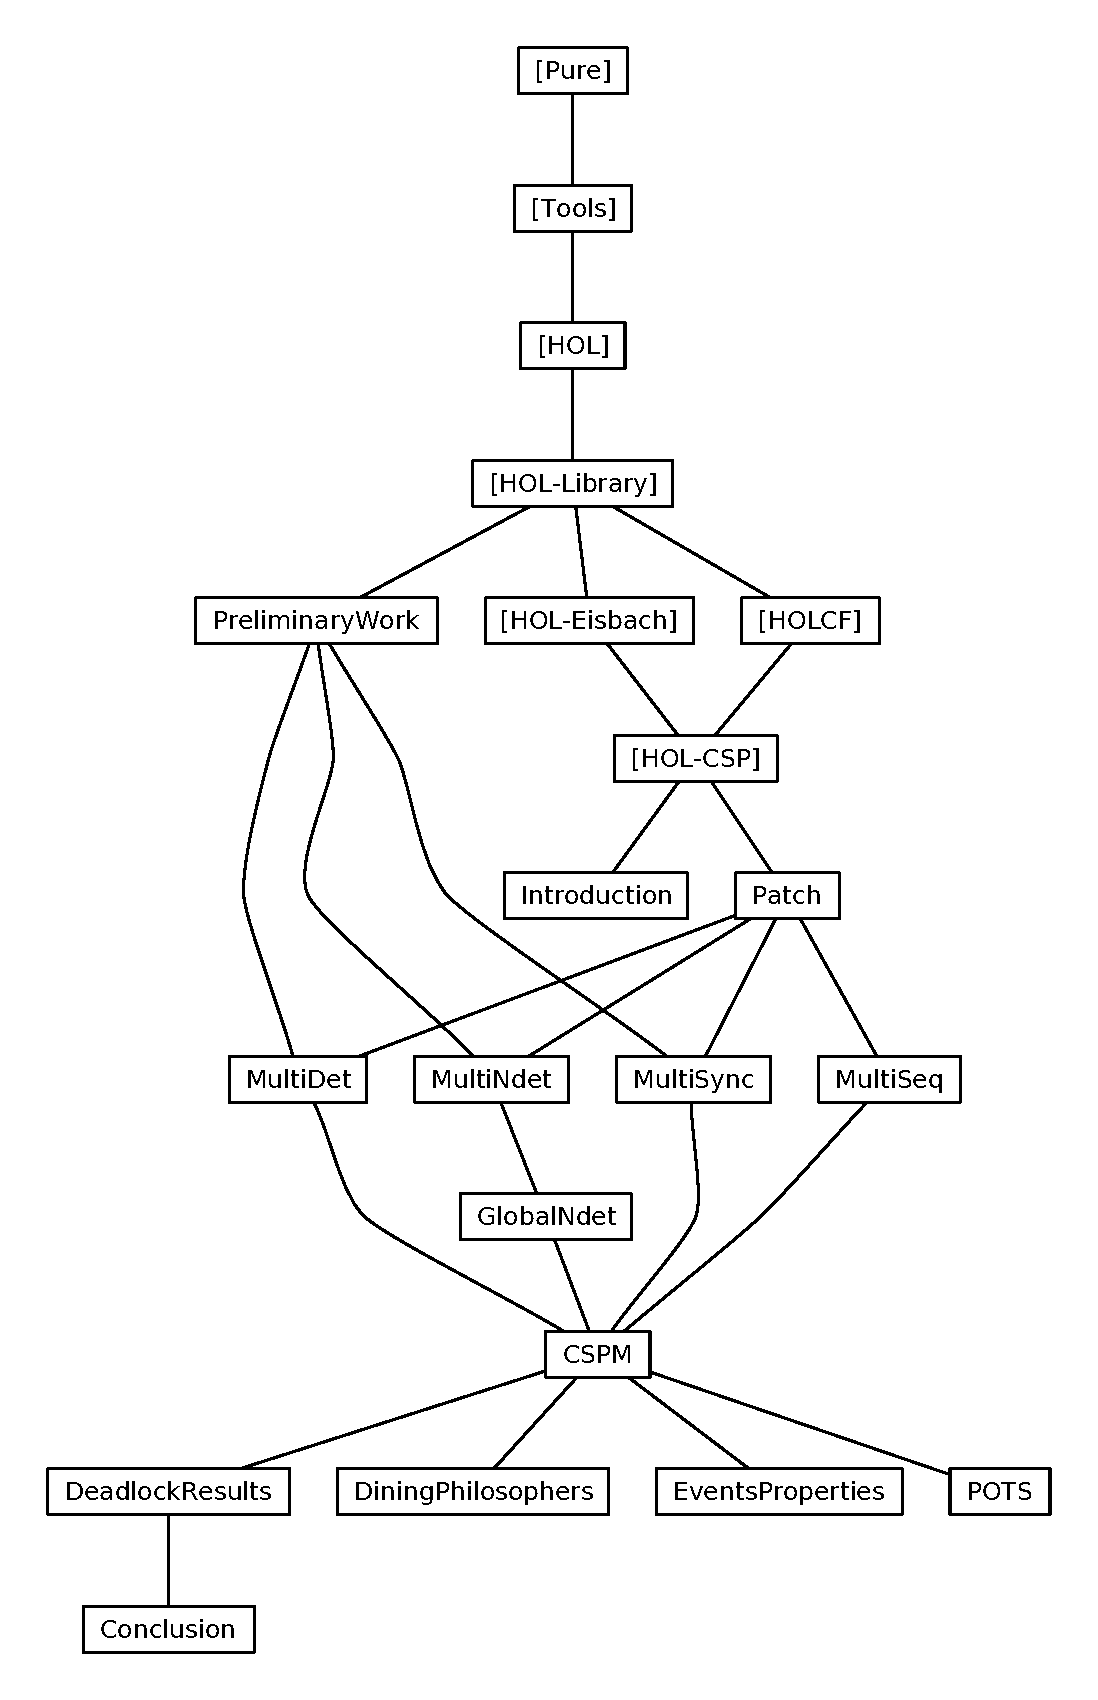
\includegraphics[scale=.7]{session_graph.pdf}
    \caption{Theory dependencies}
  \end{center}
  \label{fig:theory-dependencies}
\end{figure}



% generated text of all theories
\input{session}

% optional bibliography
%\bibliographystyle{abbrv}
%\bibliography{root}

\end{document}
